\begin{figure}[h!]
	\centering
	\resizebox {!} {8cm} {
		\begin{tikzpicture} 
			\umlclass{Play2048Player}{
				game : Play2048State\\
				search : ExpectimaxC
			}{
				+ actions() : \{\}\\
				+ play() : void
			}
			\umlclass[right=5cm of Play2048Player.east, anchor=west]{ExpectimaxC}{
				search : ctypes.CDLL \\
			}{
				+ desicion(board : Play2048State) : [] \\
			}
			\umlclass[below=6cm of ExpectimaxC.north, anchor=north]{expectimax\_c}{}{
				+ ExpectimaxNode max\_value(int* board, int depth)\\
				+ ExpectimaxNode chance\_node(int* board, int depth)\\
				+ double evaluation\_function(int* board)\\
				+ int decision(int depth, board..., double smoothness,\\\hspace{2cm} double max\_tile, double free\_tiles\_multiplier,\\\hspace{2cm} double max\_placement, double monotonicity)\\
			}
			\umlclass[below=6cm of Play2048Player.north, anchor=north]{Play2048State}{
				board : []\\
				possible\_moves : \{\}\\
				score : int
			}{
				+ perform(move : []) : Play2048State\\
				+ move(move : []) : bool\\
				+ slides(move : [], perform\_move : bool) : bool\\
				+ collision(move : [], perform\_move : bool) : bool\\
			}
			\umlunicompo[geometry=-|, stereo=game, anchors=south and north, pos stereo=1.4]{Play2048Player}{Play2048State}
			\umlunicompo[geometry=-|, stereo=search, anchors=south and north, pos stereo=1.4]{ExpectimaxC}{expectimax\_c}
			\umlunicompo[geometry=-|-, stereo=search, anchors=east and west, pos stereo=0.8]{Play2048Player}{ExpectimaxC}
		\end{tikzpicture}
	}
	\caption{Class diagram for the 2048 game task.}
\end{figure}